\colorlet{species background color}{black!15}
\tikzset{
    x={1pt},
    y={-1pt},
    species background/.style={
        fill=species background color,
        draw=species background color,
        line width={1pt},
    },
    species label/.style={
        font=\bfseries,
        midway,
        anchor=north,
        align=center,
        yshift=-10,
    },
    branch/.style={
        draw={#1},
        line width={0.5pt},
    },
    transfer branch/.style={
        branch={#1},
        -Stealth,
    },
    loss/.style={
        draw={#1}, cross out, thick,
        line width={0.5pt},
        inner sep=0pt,
        outer sep=0pt,
        minimum width={3},
        minimum height={3},
    },
    extant gene/.style 2 args={
        circle, fill={#1},
        outer sep=0pt, inner sep=0pt,
        minimum size={3},
        label={
            [font={\strut\color{#1}},
                align=center,
                inner xsep=0pt, inner ysep=2pt,
                outer xsep=0pt, outer ysep=0pt]
            below:#2
        },
    },
    extant gene/.default={black}{},
    branch node/.style={
        draw={#1}, fill={species background color!50!white},
        align=center,
        font={\color{#1}},
        outer sep=0pt, inner xsep=0pt, inner ysep=2pt,
        line width={0.5pt},
    },
    branch node/.default={black},
    speciation/.style={
        branch node={#1}, rectangle, rounded corners,
        inner xsep=4pt,
        minimum width={8},
        minimum height={8},
    },
    duplication/.style={
        branch node={#1}, rectangle,
        inner xsep=4pt,
        minimum width={8},
        minimum height={8},
    },
    horizontal gene transfer/.style={
        branch node={#1}, chamfered rectangle,
        chamfered rectangle sep={8 / 2.4},
        inner xsep=2pt,
        inner ysep=-1pt,
        minimum width={8},
        minimum height={8},
    },
}
\definecolor{reccolor0}{HTML}{000000}
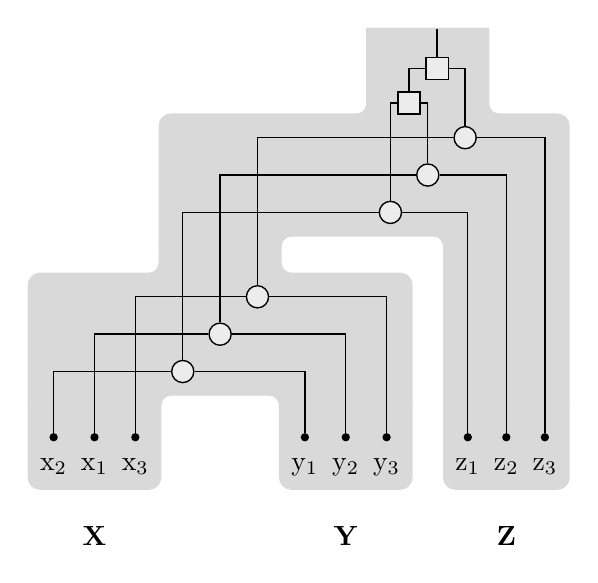
\begin{tikzpicture}
% background
\path[species background] (47.289,78.5) [rounded corners={4pt}] -- (47.289,31.0) -- (122.328,31.0) [sharp corners] -- (122.328,0) -- (165.828,0) [rounded corners={4pt}] -- (165.828,31.0) -- (194.847,31.0) [sharp corners] -- (194.847,136.0) -- (150.078,136.0) [rounded corners={4pt}] -- (150.078,74.5) -- (90.789,74.5) [sharp corners] -- (90.789,78.5) -- cycle;
\path[species background] (0,136.0) [rounded corners={4pt}] -- (0,88.5) -- (47.289,88.5) [sharp corners] -- (47.289,78.5) -- (90.789,78.5) [rounded corners={4pt}] -- (90.789,88.5) -- (138.078,88.5) [sharp corners] -- (138.078,136.0) -- (90.789,136.0) [rounded corners={4pt}] -- (90.789,132.0) -- (47.289,132.0) [sharp corners] -- (47.289,136.0) -- cycle;
\path[
                species background,
                rounded corners={4pt},
            ] (0,136.0) -- (0,166.0) -- node[species label] {X} (47.289,166.0) -- (47.289,136.0);
\path[
                species background,
                rounded corners={4pt},
            ] (90.789,136.0) -- (90.789,166.0) -- node[species label] {Y} (138.078,166.0) -- (138.078,136.0);
\path[
                species background,
                rounded corners={4pt},
            ] (150.078,136.0) -- (150.078,166.0) -- node[species label] {Z} (194.847,166.0) -- (194.847,136.0);
% species
% gene branches
\draw[branch={reccolor0}] (82.539,78.5) |- (153.328,39.25) (161.828,39.25) -| (186.3855,136.0);
\draw[branch={reccolor0}] (69.039,78.5) |- (139.828,52.75) (148.328,52.75) -| (172.4625,136.0);
\draw[branch={reccolor0}] (55.539,78.5) |- (126.328,66.25) (134.828,66.25) -| (158.5395,136.0);
\draw[branch={reccolor0}] (144.078,48.5) |- (133.078,26.75) (141.578,26.75) -| (130.578,62.0);
\path[branch={reccolor0}] (147.453,10.0) -- (147.453,0);
\draw[branch={reccolor0}] (157.578,35.0) |- (143.203,14.25) (151.703,14.25) -| (137.328,22.5);
\path[branch={reccolor0}] (82.539,92.5) -- (82.539,78.5);
\draw[branch={reccolor0}] (38.4075,136.0) |- (78.289,96.75) (86.789,96.75) -| (129.19650000000001,136.0);
\path[branch={reccolor0}] (69.039,106.0) -- (69.039,78.5);
\draw[branch={reccolor0}] (23.6445,136.0) |- (64.789,110.25) (73.289,110.25) -| (114.43350000000001,136.0);
\path[branch={reccolor0}] (55.539,119.5) -- (55.539,78.5);
\draw[branch={reccolor0}] (8.881500000000003,136.0) |- (51.289,123.75) (59.789,123.75) -| (99.6705,136.0);
\path[branch={reccolor0}] (38.407500000000006,146.0) -- (38.4075,136.0);
\path[branch={reccolor0}] (23.6445,146.0) -- (23.6445,136.0);
\path[branch={reccolor0}] (8.881499999999999,146.0) -- (8.881500000000003,136.0);
\path[branch={reccolor0}] (129.1965,146.0) -- (129.19650000000001,136.0);
\path[branch={reccolor0}] (114.43350000000001,146.0) -- (114.43350000000001,136.0);
\path[branch={reccolor0}] (99.6705,146.0) -- (99.6705,136.0);
\path[branch={reccolor0}] (186.3855,146.0) -- (186.3855,136.0);
\path[branch={reccolor0}] (172.4625,146.0) -- (172.4625,136.0);
\path[branch={reccolor0}] (158.5395,146.0) -- (158.5395,136.0);
% gene transfers
% events
\node[speciation={reccolor0}] at (157.578,39.25) {};
\node[speciation={reccolor0}] at (144.078,52.75) {};
\node[speciation={reccolor0}] at (130.578,66.25) {};
\node[duplication={reccolor0}] at (137.328,26.75) {};
\node[duplication={reccolor0}] at (147.453,14.25) {};
\node[speciation={reccolor0}] at (82.539,96.75) {};
\node[speciation={reccolor0}] at (69.039,110.25) {};
\node[speciation={reccolor0}] at (55.539,123.75) {};
\node[extant gene={reccolor0}{x\textsubscript{3}}] at (38.407500000000006,147.5) {};
\node[extant gene={reccolor0}{x\textsubscript{1}}] at (23.6445,147.5) {};
\node[extant gene={reccolor0}{x\textsubscript{2}}] at (8.881499999999999,147.5) {};
\node[extant gene={reccolor0}{y\textsubscript{3}}] at (129.1965,147.5) {};
\node[extant gene={reccolor0}{y\textsubscript{2}}] at (114.43350000000001,147.5) {};
\node[extant gene={reccolor0}{y\textsubscript{1}}] at (99.6705,147.5) {};
\node[extant gene={reccolor0}{z\textsubscript{3}}] at (186.3855,147.5) {};
\node[extant gene={reccolor0}{z\textsubscript{2}}] at (172.4625,147.5) {};
\node[extant gene={reccolor0}{z\textsubscript{1}}] at (158.5395,147.5) {};
\end{tikzpicture}
